\section{Experiments on SPO-tree}
\label{sec:experiments_on_spo_tree}

\textbf{Experimental Setups.}
To evaluate our method in long CoT scenario, we utilize DeepSeek-R1-Distill-Qwen-1.5B model as our base model, which has been fine-tuned on huge amount of long CoT data, demonstrating complex reasoning strategies and typically generating long outputs. Given the strong capability of these models, we select the competition-level MATH \cite{hendrycks2021measuringmathematicalproblemsolving} dataset for our training and evaluation. We mainly focus on comparing our proposed SPO-tree method against GRPO, as GRPO is the mainstream training approach adopted for reasoning models, particularly favored for long CoT scenarios due to its efficiency. We do not compare with VinePPO because its efficiency issue, making it impractical to apply in long CoT settings. For our SPO-tree method, the structure remains identical to the SPO-tree used in the short CoT scenario, as described in Section \ref{sec:experiments_on_spo_chain}. Detailed hyper-parameters can be found in Appendix \ref{appendix:hyperparameter}.

\textbf{Comparison with Baseline Methods.}
We initially limit the training context window size to 2K and evaluate model accuracy (Pass@1) on MATH500 every 10 iterations. For evaluation, we follow the implementation provided by \cite{kazemnejad2024vineppounlockingrlpotential}, setting the evaluation context window also to 2K and using greedy decoding (temperature = 0). Figure \hyperref[fig:SPO-tree-results]{5(a)} shows the training curves of SPO-tree, vanilla GRPO, and GRPO with probability mask. We observe that GRPO with probability-mask outperforms vanilla GRPO to some extent, demonstrating the effectiveness of this technique in long CoT scenarios. However, SPO-tree still achieves significantly higher accuracy under the same wall-clock time. This validates the effectiveness of SPO-tree and highlights that introducing segment advantage values is crucial for achieving better performance.

To further assess our method, we continue training from the 2K checkpoint and expand the model's context length to 4K. The corresponding model performance is presented in Table \ref{tab:context_accuracy}. We adopt the evaluation script provided by \cite{openr1}  to conduct evaluation on the obtained model checkpoints. As shown in the results, the SPO-tree consistently outperforms GRPO across all context sizes and achieves superior performance under 2K and 4K contexts, which are the context lengths it was trained on. We hypothesize that our segment-level advantage method significantly increases token efficiency due to more precise credit assignment, enabling the model to arrive at correct answers more straightforwardly (see Appendix \ref{appendix:model_output_example}). This improvement leads to considerably better performance under limited context sizes. Interestingly, even though our model is trained under context windows up to 4K, it still achieves improved performance under 32K context evaluation, surpassing the base model. We also compared our approach against the most recent works, including DeepScaleR \cite{deepscaler2025} and STILL-3 \cite{Slow_Thinking_with_LLMs_3}, both of which were trained on DeepSeek-R1-Distill-Qwen-1.5B using GRPO. Notably, DeepScaleR and STILL-3 adopted larger training datasets and extended context windows for training. Specifically, DeepScaleR progressively increased the context length from 8K to 16K and finally to 24K, whereas our training scales only from 2K to 4K. While DeepScaleR performs best at 32K, we observe the opposite trend in lower-context settings, where DeepScaleR exhibits the worst performance at 2K and 4K. This finding suggests that GRPO-based training might not optimize token efficiency, potentially leading to redundancy in the generated outputs, and thus negatively affecting the model’s performance when evaluated under limited context size. 

\begin{figure}[t]
    \centering
    \begin{minipage}[t]{0.32\textwidth}
        \centering
        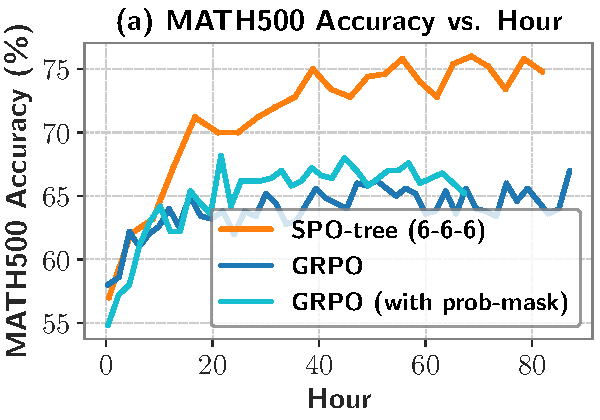
\includegraphics[width=\textwidth]{eval-figures/SPO-tree-GRPO-line-LoT.pdf}
    \end{minipage}%
    \hfill
    \begin{minipage}[t]{0.32\textwidth}
        \centering
        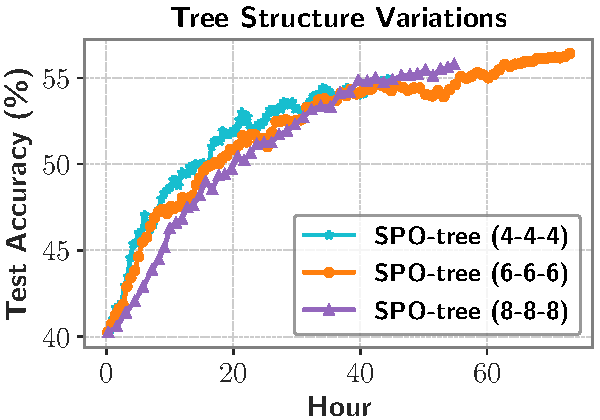
\includegraphics[width=\textwidth]{eval-figures/SPO-tree-structure-var.pdf}
    \end{minipage}
    \hfill
    \begin{minipage}[t]{0.32\textwidth}
        \centering
        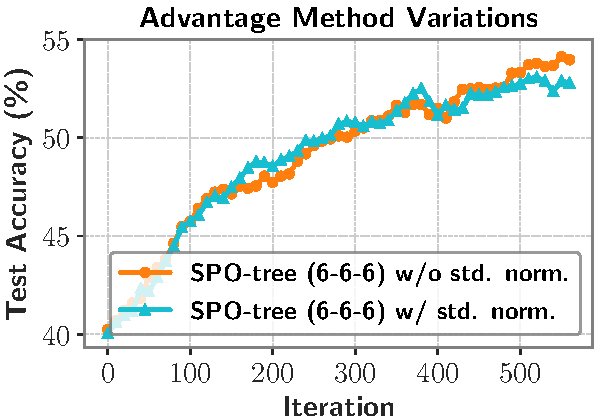
\includegraphics[width=\textwidth]{eval-figures/SPO-tree-policy-var.pdf}
    \end{minipage}
     \caption{\textbf{(a)} Comparison of SPO-tree (6-6-6) and GRPO on MATH500 with a context size of 2K. \textbf{(b)} Variations of  tree structures on GSM8K. \textbf{(c)} SPO-tree with different advantage methods on GSM8K.}
     \label{fig:SPO-tree-results}
\end{figure}


\begin{table}[t]
\centering
\small
\begin{threeparttable}

    \begin{tabular}{ccccc|cc}
        \toprule
        \textbf{Dataset} & \textbf{Eval Context Size} & \textbf{Base} & \textbf{GRPO} & \textbf{SPO-tree} & \textbf{DeepScaleR\tnote{*}} & \textbf{STILL-3\tnote{*}} \\
        \midrule
        \multirow{3}{*}{MATH500} & 2K   & 0.566 & 0.62  & \textbf{0.736} & 0.538 & 0.662 \\
                                 & 4K   & 0.74  & 0.752 & \textbf{0.828} & 0.744 & 0.794 \\
                                 & 32K  & 0.838 & 0.84  & 0.848          & \textbf{0.878} & 0.846 \\

        \midrule
        \multirow{3}{*}{AIME24} & 2K    & 0.067    & 0.033    & \textbf{0.1}             & 0    & 0.067    \\
                                & 4K    & 0.167    & \textbf{0.2}    & \textbf{0.2}             & 0.167    & 0.133    \\
                                & 32K   & 0.267 & \textbf{0.333} & \textbf{0.333}          & \textbf{0.333} & 0.233 \\
\bottomrule
\end{tabular}
  \begin{tablenotes}
    \item[*] \textbf{These models were trained using larger datasets and longer context windows}. Specifically, DeepScaleR uses 8K$\to$16K$\to$24K context and STILL-3 sets `generate\_max\_len' to 29000 during training, while our GRPO and SPO-tree use a maximum context of 4K during training.
  \end{tablenotes}

\end{threeparttable}

\vspace{1em}
\caption{Accuracy comparison among methods with various context sizes on MATH500 and AIME24.}
\label{tab:context_accuracy}
\vspace{-0.5cm}
\end{table}

\textbf{Comparison of Different Tree Structures and Advantage Computation Methods.} 
To investigate the impact of different tree structures, we compared the performance\footnote{Evaluation time is also included in the reported wall-clock time. The model is evaluated every 10 iterations.} of various tree structures (4-4-4, 6-6-6, 8-8-8) on the GSM8K test set (Figure \hyperref[fig:SPO-tree-results]{5(b)}). When using a larger tree structure, each iteration generates a greater number of segments with non-zero advantage. Therefore, we set different values of the hyperparameter "num\_episodes\_per\_iteration" for different tree structures: specifically, we set it to 1024 for SPO-tree (8-8-8), 512 for SPO-tree (6-6-6), and 384 for SPO-tree (4-4-4). We found that the performance differences among these tree structures were not substantial under the same wall-clock time, indicating the robustness of the tree structure. Smaller tree structures achieve higher accuracy initially, possibly because they can process more data examples within the same time frame. However, larger tree structures eventually outperform smaller ones at later training stages, as they enable more accurate value estimation and benefit from having more segments within each group, leading to more reliable and nuanced advantage estimates. We also compared the performance of different advantage calculation methods with and without standard deviation normalization. As shown in Figure \hyperref[fig:SPO-tree-results]{5(c)}, both methods perform similarly, while the variant without normalization performs slightly better.
